\subsection{Activation}

The activation calculations are performed in several steps as described in the sections below:
\begin{enumerate}
  \item Prepare geometry.
  \item Calculate neutron fluxes. \\
    These first two runs are completely independent, but they must use the same model. 
    Normally the difference between them is that the second run has the energy cut, while the first~--- not.
    In principle we do not need the energy cut, but it saves time.
  \item Generate spalation products in the {\tt htape} files with {\tt MCNPX}.
\end{enumerate}
\subsubsection{Geometry}
In this particular example we are going to look at a chopper
of the  {\tt BIRFOST} beam line: how active will the chopper beam
port become when we try to take it off?\footnote{I.e. the rotors and motors are lifted out (with a crane) and we are left with the chopper housing.} In other words, we will calculate residual dose and gamma spectra.

First, we will build the {\tt BIFROST} geometry and rotate it around
its axis\footnote{The {\tt bifrostStopPoint} argument is described in \secrefp{sec:model:ess:beam-lines:StopPoint}.}:

\begin{bash}
./ess -r -defaultConfig Single BIFROST -angle objAxis bifrostAxis 0 \
      -v bifrostStopPoint 3 \
      ChopA
\end{bash}

The beam line geometry is shown in \figref{fig:activation:bifrost:geometry}.

\begin{figure}
  \centering
  \subfloat[MCNPX: horizontal cut through the beam line]{
    \begin{tikzpicture}
      \node[anchor=south west,inner sep=0] (image) at (0,0) {
        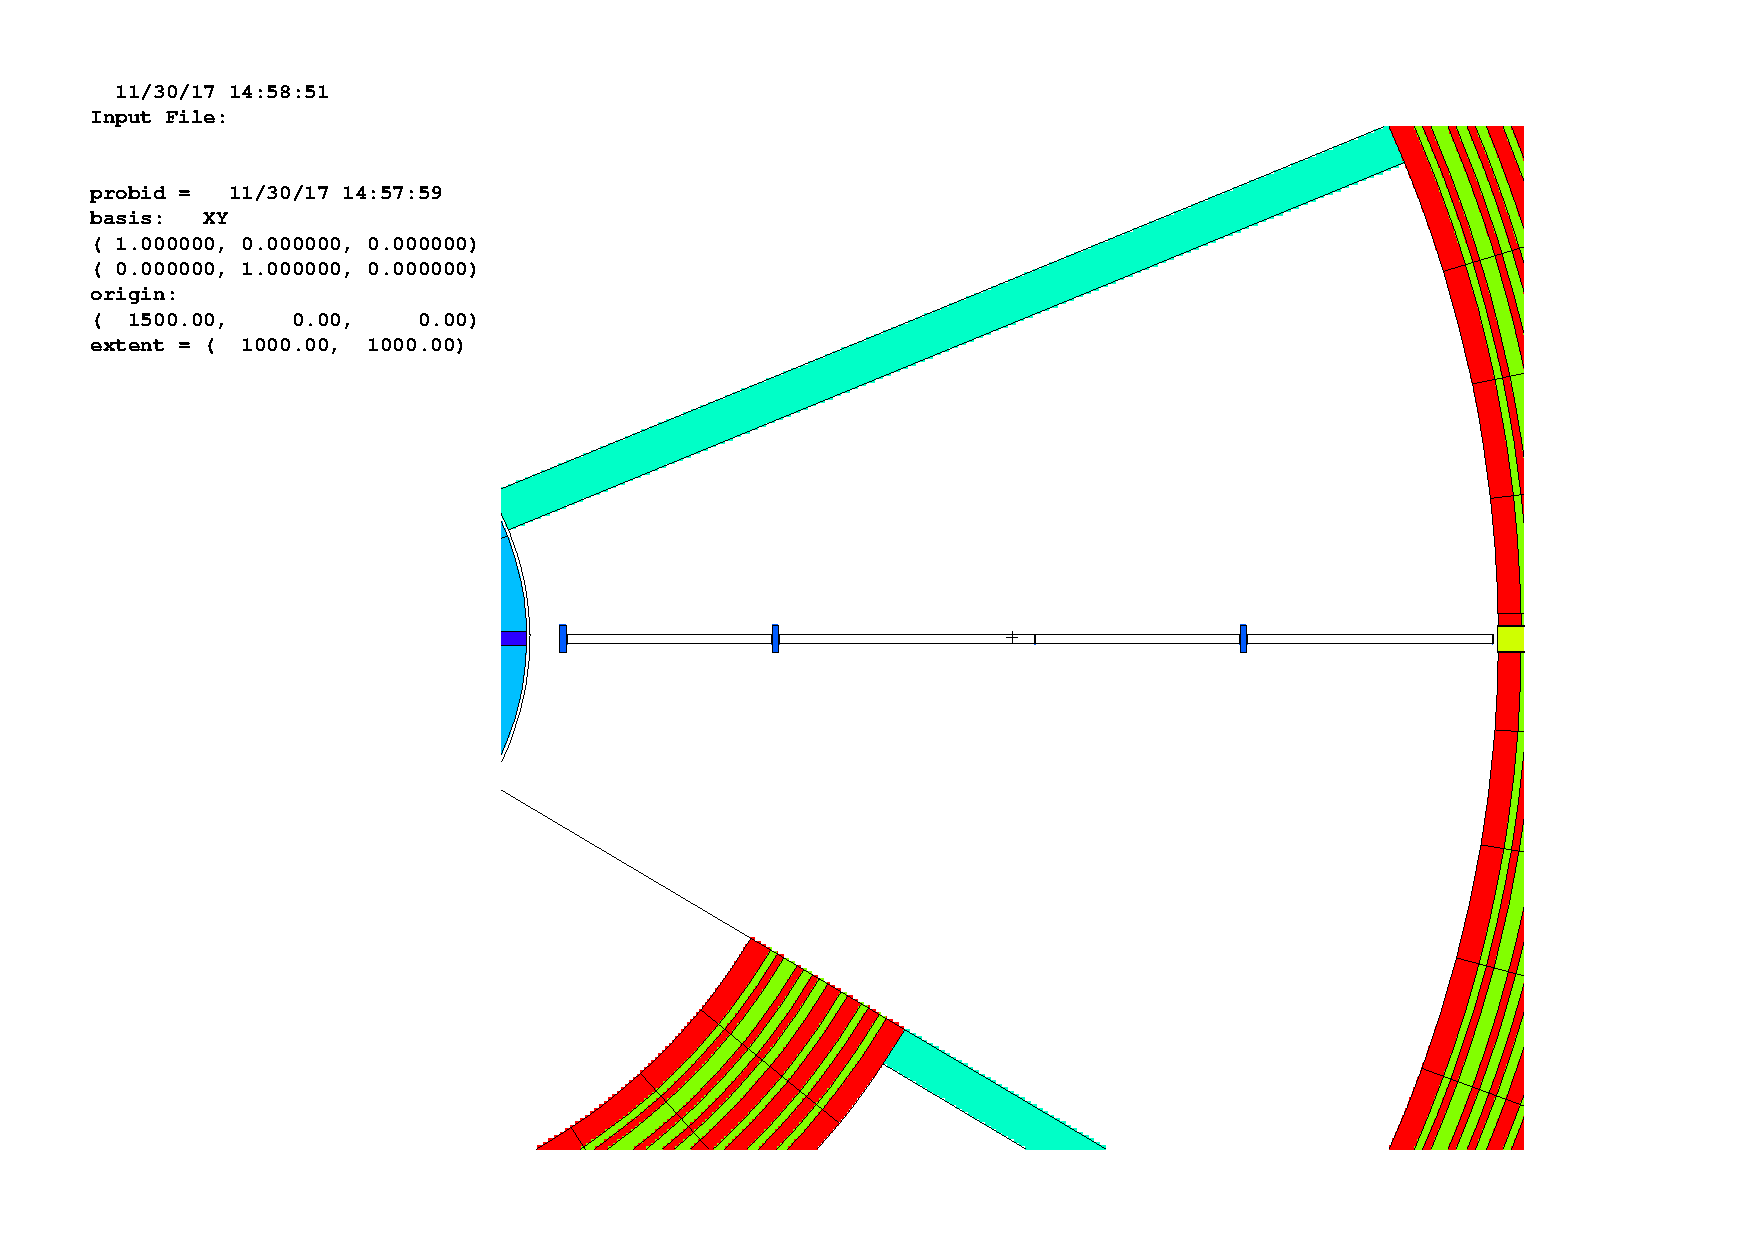
\includegraphics[height=0.28\textheight,clip=true, trim=8.5cm 2cm 4cm 3cm]{UserGuide/activation/bifrost.pdf}};
      \begin{scope}[x={(image.south east)},y={(image.north west)}]
        % \draw[help lines, xstep=.1, ystep=.1] (0,0) grid (1,1);
        % \foreach \x in {0,1,...,9} {\node [anchor=north] at (\x/10, 0) {0.\x}; }
        % \foreach \y in {0,1,...,9} {\node [anchor=east]  at (0, \y/10) {0.\y}; }

         \draw[arrow] (0.06,0.36) -- (0.06, 0.48); \node[legend] at (0.06,0.36) {Chopper\,A};
         \draw[arrow] (0.27,0.36) -- (0.27, 0.48); \node[legend] at (0.27,0.36) {Chopper\,B};
         \draw[arrow] (0.728,0.36) -- (0.728, 0.48); \node[legend] at (0.728,0.36) {Chopper\,C};
        \end{scope}
      \end{tikzpicture}
    }
  \quad
  \subfloat[Same geometry rendered with POV-Ray]{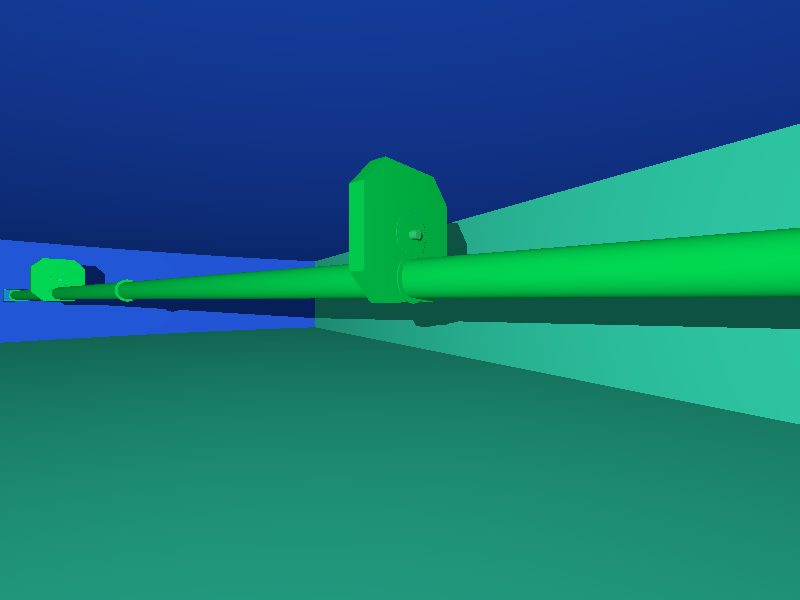
\includegraphics[height=0.28\textheight]{UserGuide/activation/bifrost.png}}
  \caption{Geometry of the {\tt BIFROST} beam line inside Bunker}
  \label{fig:activation:bifrost:geometry}
\end{figure}

\subsubsection{Neutron fluxes}
Now we need to set up neutron flux {\tt f4} tallies in all non-void cells of ports {\tt A} and {\tt B} of the chopper {\tt A}
(see geometry in \figref{fig:activation:bifrost:geometry:chopperA}):
\lstinputlisting[language=bash,numbers=none,backgroundcolor=\color{yellow!20},frame=tb]{UserGuide/activation/buildCollA.sh}

\begin{figure}
  \centering
  \begin{tikzpicture}
    \node[anchor=south west,inner sep=0] (image) at (0,0) {
      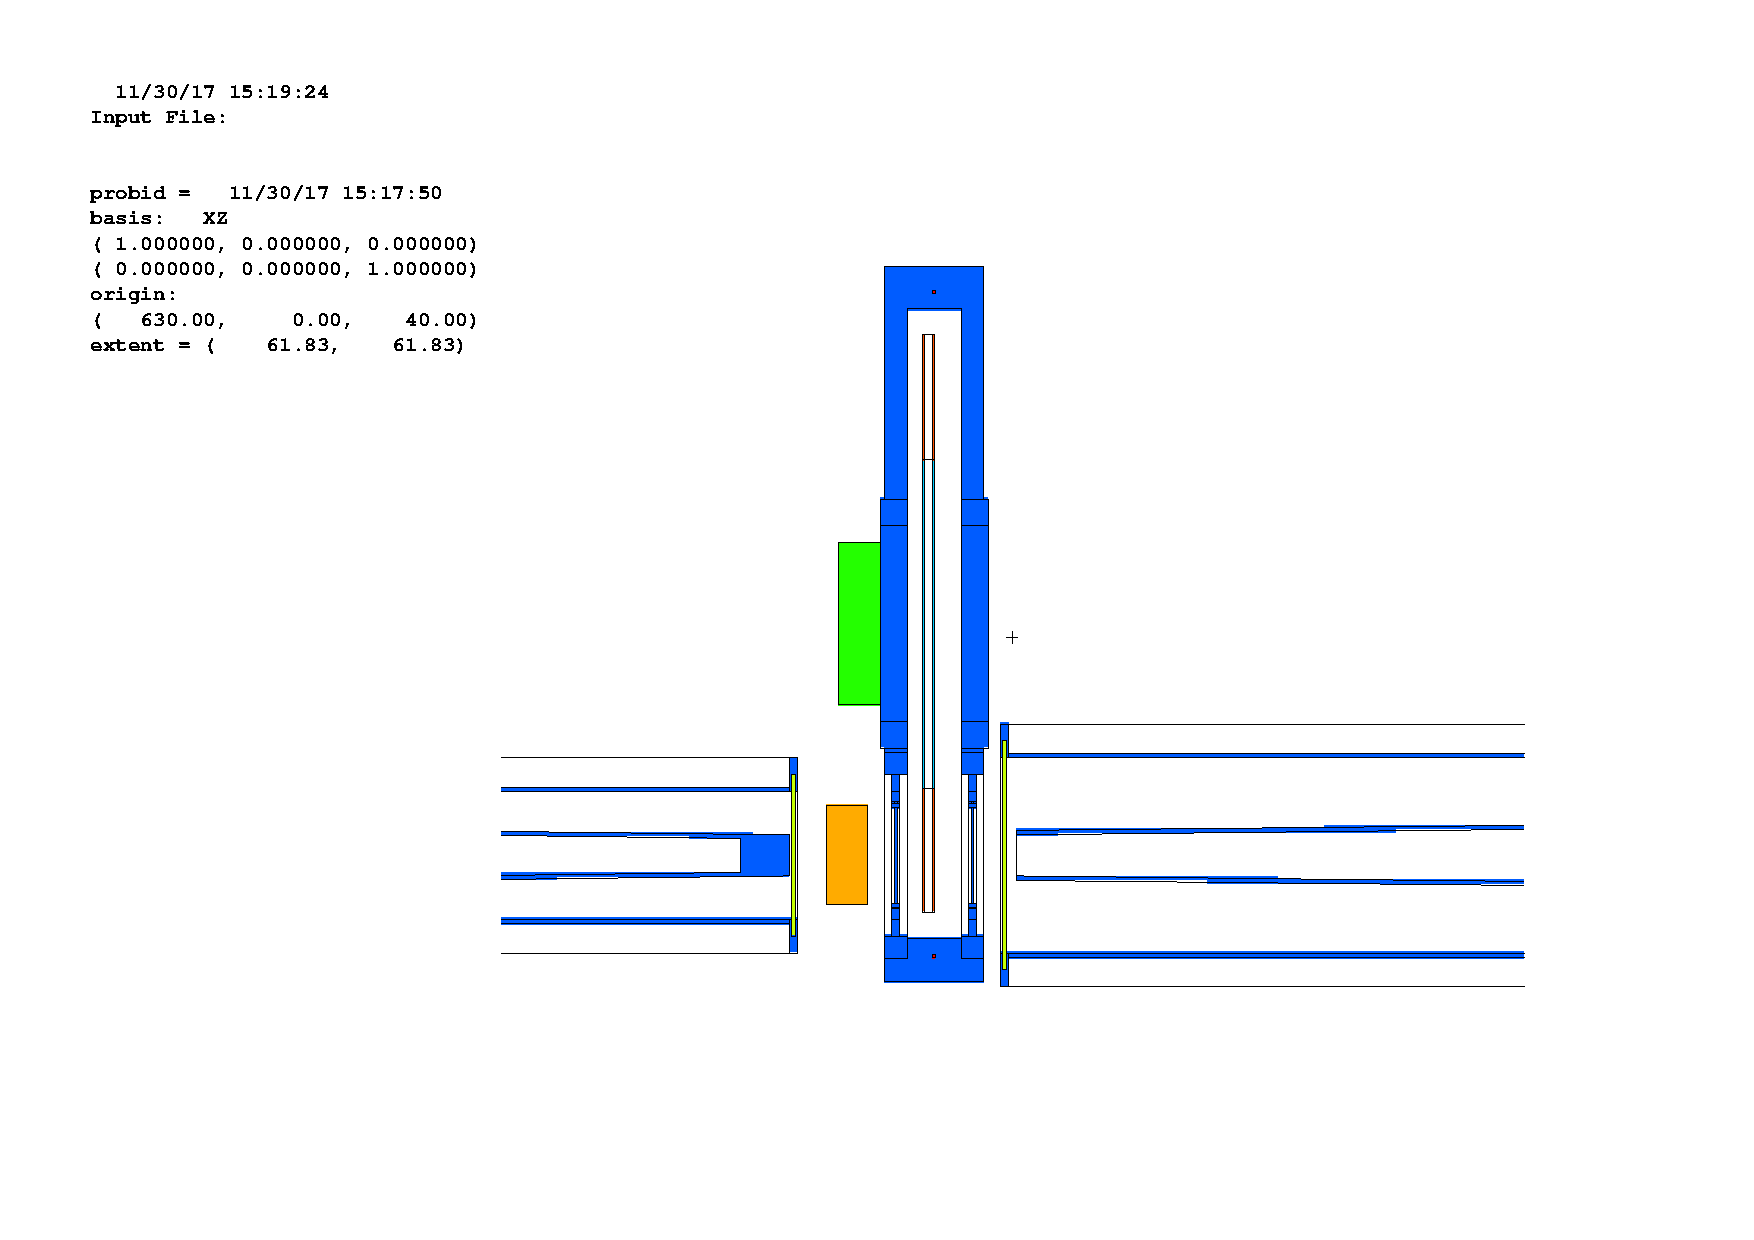
\includegraphics[width=\textwidth,clip=true, trim=8.5cm 2cm 4cm 3cm]{UserGuide/activation/bifrost-chopperA.pdf}};
    \begin{scope}[x={(image.south east)},y={(image.north west)}]
      % \draw[help lines, xstep=.1, ystep=.1] (0,0) grid (1,1);
      % \foreach \x in {0,1,...,9} {\node [anchor=north] at (\x/10, 0) {0.\x}; }
      % \foreach \y in {0,1,...,9} {\node [anchor=east]  at (0, \y/10) {0.\y}; }
      
      \draw[arrow] (0.3,0.1) -- (0.38, 0.25); \node[legend] at (0.3,0.1) {Port\,A};
      \draw[arrow] (0.55,0.1) --(0.47, 0.25); \node[legend] at (0.55,0.1) {Port\,B};
    \end{scope}
  \end{tikzpicture}
  \caption{Geometry of the {\tt BIFROST} chopper A}
  \label{fig:activation:bifrost:geometry:chopperA}
\end{figure}

The {\tt -cinder} argument does two things:
\begin{itemize}
\item adds the {\tt histp} card with all the cells listed in both {\tt f4} tallies.
  (if you want just {\tt histp} cards, use the {\tt -histp} argument.)
\item creates a file called {\tt materials} with material definitions later used by \alert{whom}?
\end{itemize}
The default energy bins generated by the {\tt -T flux} cards already match the \cinder binning.

The {\tt -TMod single -4} arguments remove brackets around the cells used in all {\tt f4} tallies.
{\tt -4} means `all {\tt f4} tallies', while
{\tt 4} would mean 'only {\tt f4} tally'.

Of course, for {\tt MCNPX} simulations this flag is needed: {\tt -mcnp 10}.
You need to have neutron fluxes with good statistics, therefore it is advised to use variance reduction (see \secrefp{sec:vr}).

\begin{quote}
You need to fix the \mcnp\ {\tt source.F} file to correct velocity and cell finding error and allow to start SSR not at a surface.

SA puts bounding box of neutrons to come in out of a beam port and then he restarts those neutrons within this box.
Convenient thing is that in the new geometry the surface numbers may change (as they always do with CombLayer), but
this fix allows SSR start particles from a bounding box not caring about surface numbers\footnote{I.e. the SSW and SSR cards do not have to have the same surface numbers.}.
\end{quote}

\subsubsection{htape}
Second run generates the {\tt htape} file:
\lstinputlisting[language=bash,numbers=none,backgroundcolor=\color{yellow!20},frame=tb]{UserGuide/activation/buildCollHA.sh}
You do not need it if you do not care about spallation reactions.

The energy cut {\tt -C 0.1} needs in order to speed up since we get particles only from histp.
{\tt -mcnp 10} is needed since we are going to generate {\tt htape} with {\tt MCNPX}.

\subsubsection{Activation script}

\href{https://github.com/SAnsell/CombLayer\_Activation}{https://github.com/SAnsell/CombLayer\_Activation}

Now we have to prepare the activation script input file. Its syntax is similar to the \cinder one (inpact), but much more forgiving.
We call it {\tt bifrostStop01}:
\lstinputlisting[numbers=none,backgroundcolor=\color{yellow!20},frame=tb]{UserGuide/activation/bifrostStop01}

Lines can be concatenated by backslash. The order of keywords in the given section does not matter.

\begin{description}
  \item[title\_lines] as many lines as necessary are possible. Everything longer 72 characters is chopped.
  \item[mat\_file] materials. Normally one of the MCNP output files
   \item[mcnpx\_outp] list of all the files you wish to sum together. Wild-masks and directories are supported.
   \item[mcnpx\_histp] list of {\tt histp} files
   \item[htape\_exe] htape3x
   \item[cinder\_exe] cinder
   \item[tabcode\_exe] tabcode
   \item[library] CINDER libs
\end{description}